% Evaluation section body (\input from qshieldx.tex). Every number is a \claim backed by results/.

\subsection{Software baselines: accuracy}\label{sec:eval-pl}
Figure~\ref{fig:pl} shows P\textsubscript{L} per $d$-round block for PyMatching and both QSX-UF variants over
$p\in[0.001,0.01]$ and $d\in\{3,5,7,9\}$. Each point runs until a target number of failures or a shot cap is reached,
and carries an exact Clopper--Pearson 95\% interval \stage{Monte Carlo, Stim}. At $p=0.003$, weighted QSX-UF
has P\textsubscript{L} $=\claim{M1_PL_d7_p003_UF}$ against $\claim{M1_PL_d7_p003_PM}$ for PyMatching at $d=7$
(ratio \claim{M1_ratio_d7_p003}), and $\claim{M1_PL_d9_p003_UF}$ against $\claim{M1_PL_d9_p003_PM}$ at $d=9$ (ratio
\claim{M1_ratio_d9_p003}). The $d=7/9$ curve crossings are at $p\approx\claim{M1_thr_UF_7_9}$ (QSX-UF) and
\claim{M1_thr_PM_7_9} (PyMatching). The 3-bit weights are essential: the unweighted variant is markedly worse at large
$d$ (Fig.~\ref{fig:pl}, right panel). The accuracy gap is the price of the order-independent, hardware-friendly
algorithm, and it grows with distance.

\begin{figure}[t]\centering
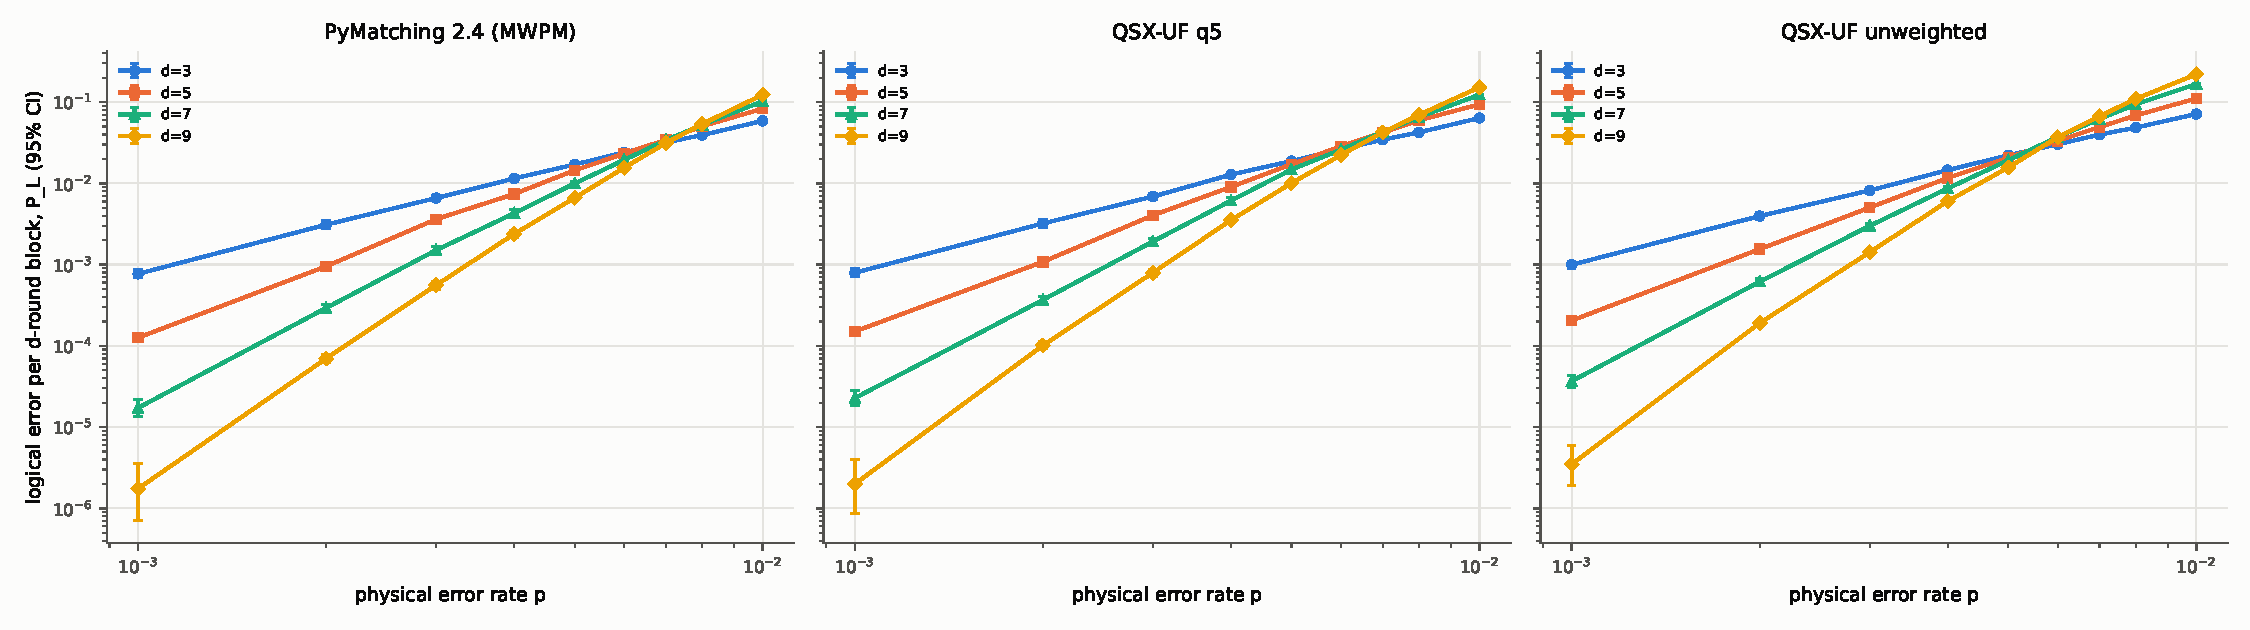
\includegraphics[width=\linewidth]{M1/figs/pl_vs_p.pdf}
\caption{P\textsubscript{L} vs.\ physical error rate (95\% CIs), circuit-level depolarizing noise, $d$ rounds.}
\label{fig:pl}
\end{figure}

\subsection{RTL correctness: co-simulation}
% AUTO-GENERATED by bench/claims_ext.py -- do not edit
\begin{table}[t]\centering\small
\caption{Co-simulation of the final RTL against the C++ golden model (status, rounds, observable, full correction bitmap and cycle count compared per syndrome). Columns: syndromes / mismatches.}
\label{tab:cosim}
\begin{tabular}{lrrrrrr}\toprule & \multicolumn{2}{c}{$d=3$} & \multicolumn{2}{c}{$d=5$} & \multicolumn{2}{c}{$d=7$} \\ \midrule
\claim{M2_ct_corerandom_lab} & \claim{M2_ct_corerandom_d3_sy} & \claim{M2_ct_corerandom_d3_mi} & \claim{M2_ct_corerandom_d5_sy} & \claim{M2_ct_corerandom_d5_mi} & \claim{M2_ct_corerandom_d7_sy} & \claim{M2_ct_corerandom_d7_mi} \\
\claim{M2_ct_corestim_lab} & \claim{M2_ct_corestim_d3_sy} & \claim{M2_ct_corestim_d3_mi} & \claim{M2_ct_corestim_d5_sy} & \claim{M2_ct_corestim_d5_mi} & \claim{M2_ct_corestim_d7_sy} & \claim{M2_ct_corestim_d7_mi} \\
\claim{M2_ct_sweep_lab} & \claim{M2_ct_sweep_d3_sy} & \claim{M2_ct_sweep_d3_mi} & \claim{M2_ct_sweep_d5_sy} & \claim{M2_ct_sweep_d5_mi} & \claim{M2_ct_sweep_d7_sy} & \claim{M2_ct_sweep_d7_mi} \\
\claim{M2_ct_toprandomstress_lab} & \claim{M2_ct_toprandomstress_d3_sy} & \claim{M2_ct_toprandomstress_d3_mi} & \claim{M2_ct_toprandomstress_d5_sy} & \claim{M2_ct_toprandomstress_d5_mi} & \claim{M2_ct_toprandomstress_d7_sy} & \claim{M2_ct_toprandomstress_d7_mi} \\
\claim{M2_ct_topstimstress_lab} & \claim{M2_ct_topstimstress_d3_sy} & \claim{M2_ct_topstimstress_d3_mi} & \claim{M2_ct_topstimstress_d5_sy} & \claim{M2_ct_topstimstress_d5_mi} & \claim{M2_ct_topstimstress_d7_sy} & \claim{M2_ct_topstimstress_d7_mi} \\
\bottomrule\end{tabular}\end{table}

Table~\ref{tab:cosim} summarises the campaign on the final RTL: \claim{M2_cosim_total} syndromes, with
\claim{M2_cosim_mm} mismatches in status, round count, observable, full correction bitmap or cycle count. The
shell runs inject malformed frames and incomplete configuration sessions. Every malformed frame was answered with
\texttt{FRAME\_ERROR} and every frame after an incomplete session with \texttt{CFG\_INVALID}, in order, as the
model predicts.

\subsection{Hardware: cycles, resources and latency}\label{sec:eval-hw}
TODO-hw

\subsection{Cost of the verified mechanisms}
Table~\ref{tab:overhead} separates the decoder core from the verified shell with a hierarchical synthesis
\stage{synth}. The shell contains the commit-on-last frame FIFO (backpressure, I1/P3), the atomic configuration
session with its written-word bitmap and range check (P5/P6), and the dispatcher, round-tag path and status gating
(P1--P4). At $d=5$ it costs \claim{M3_shell_lut_d5} LUT4 against \claim{M3_core_lut_d5} for the core
(\claim{M3_shell_lut_pct_d5}\%), but \claim{M3_shell_ff_pct_d5}\% of the flip-flops. Most of those FFs hold the
threshold table, which any configurable decoder needs; the atomicity bookkeeping itself is one bit per configuration
word plus one range-error bit. In time, framing and the handshakes add \claim{M3_shell_cycles_d3},
\claim{M3_shell_cycles_d5} and \claim{M3_shell_cycles_d7} cycles per frame at $d=3,5,7$ \stage{sim}: the input
header and syndrome beats, the dispatcher's load and the output header. Formal-only logic sits under
\texttt{ifdef FORMAL} and is not synthesised.
% AUTO-GENERATED by bench/claims_ext.py -- do not edit
\begin{table}[t]\centering\small
\caption{Core vs.\ verified shell (Yosys \texttt{synth\_ecp5 -noflatten}, LANES=8) and the shell's framing/handshake cycles per frame (Verilator, one frame in flight).}
\label{tab:overhead}
\begin{tabular}{lrrrrrrrr}\toprule & \multicolumn{3}{c}{core} & \multicolumn{3}{c}{shell} & & \\ & LUT4 & FF & BRAM & LUT4 & FF & BRAM & shell LUT & cycles \\ \midrule
$d=3$ & \claim{M3_core_lut_d3} & \claim{M3_core_ff_d3} & \claim{M3_core_bram_d3} & \claim{M3_shell_lut_d3} & \claim{M3_shell_ff_d3} & \claim{M3_shell_bram_d3} & \claim{M3_shell_lut_pct_d3}\% & \claim{M3_shell_cycles_d3} \\
$d=5$ & \claim{M3_core_lut_d5} & \claim{M3_core_ff_d5} & \claim{M3_core_bram_d5} & \claim{M3_shell_lut_d5} & \claim{M3_shell_ff_d5} & \claim{M3_shell_bram_d5} & \claim{M3_shell_lut_pct_d5}\% & \claim{M3_shell_cycles_d5} \\
\bottomrule\end{tabular}\end{table}


\subsection{WebAssembly runtime and the V8 patch}\label{sec:eval-wasm}
TODO-wasm

\subsection{Extensions}\label{sec:ext}
TODO-ext
